% Template for PLoS
% Version 1.0 January 2009
%
% To compile to pdf, run:
% latex plos.template
% bibtex plos.template
% latex plos.template
% latex plos.template
% dvipdf plos.template

\documentclass[10pt]{article}

% amsmath package, useful for mathematical formulas
\usepackage{amsmath}
% amssymb package, useful for mathematical symbols
\usepackage{amssymb}

% graphicx package, useful for including eps and pdf graphics
% include graphics with the command \includegraphics
\usepackage{graphicx,multirow}

% cite package, to clean up citations in the main text. Do not remove.
\usepackage{cite}

\usepackage{color}

% Use doublespacing - comment out for single spacing
%\usepackage{setspace}
%\doublespacing


% Text layout
\topmargin 0.0cm
\oddsidemargin 0.5cm
\evensidemargin 0.5cm
\textwidth 16cm
\textheight 21cm

% Bold the 'Figure #' in the caption and separate it with a period
% Captions will be left justified
\usepackage[labelfont=bf,labelsep=period,justification=raggedright]{caption}

% Use the PLoS provided bibtex style
\bibliographystyle{plos2009}

% Remove brackets from numbering in List of References
\makeatletter
\renewcommand{\@biblabel}[1]{\quad#1.}
\makeatother


% Leave date blank
\date{}

\pagestyle{myheadings}
%% ** EDIT HERE **


%% ** EDIT HERE **
%% PLEASE INCLUDE ALL MACROS BELOW
% Comments for making sure we touch all the bases for a good paper
\newif\ifcommentsw
\commentswtrue
\newcommand{\comment}[1]{\ifcommentsw  $\blacktriangleright$\ \textbf{#1}\ $\blacktriangleleft$ \fi}
%\commentswfalse   % remove the % to remove informational comments


% Notes on the paper for communicating with coauthors
\newif\ifnotesw
\noteswtrue
\newcommand{\notes}[1]{\ifnotesw  $\bullet$\ \textit{ \textbf{#1}}\ $\bullet$ \fi}
%\noteswfalse   % remove the % to remove notes to coauthors

\newcommand{\br}{\mathbf{r}}
\newcommand{\sgn}{\operatorname{sgn}}
\def\cq{{\textit{Culex quinquefasciatus}}}

%% END MACROS SECTION

\begin{document}

\begin{figure}[!htp]
% 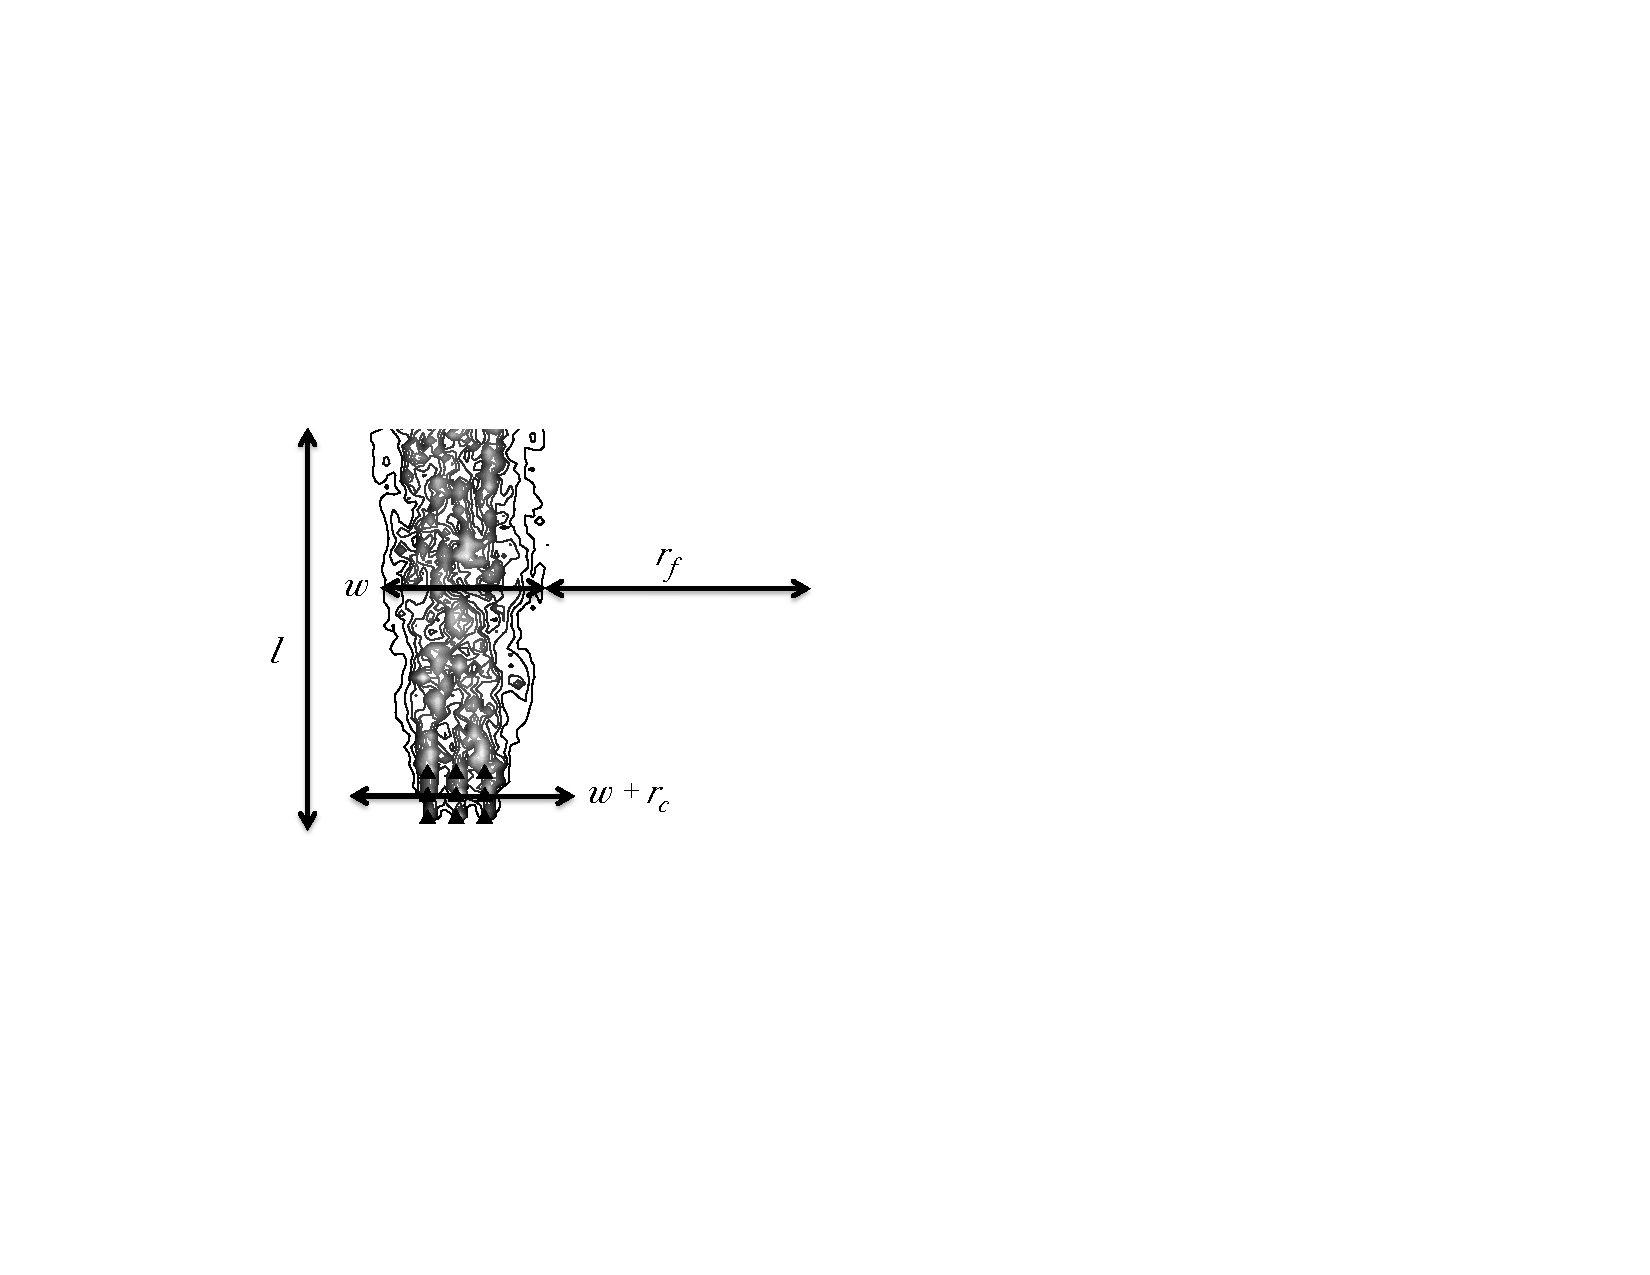
\includegraphics[width=3.25in]{revisedfigures/SupplMatFig1A}
% 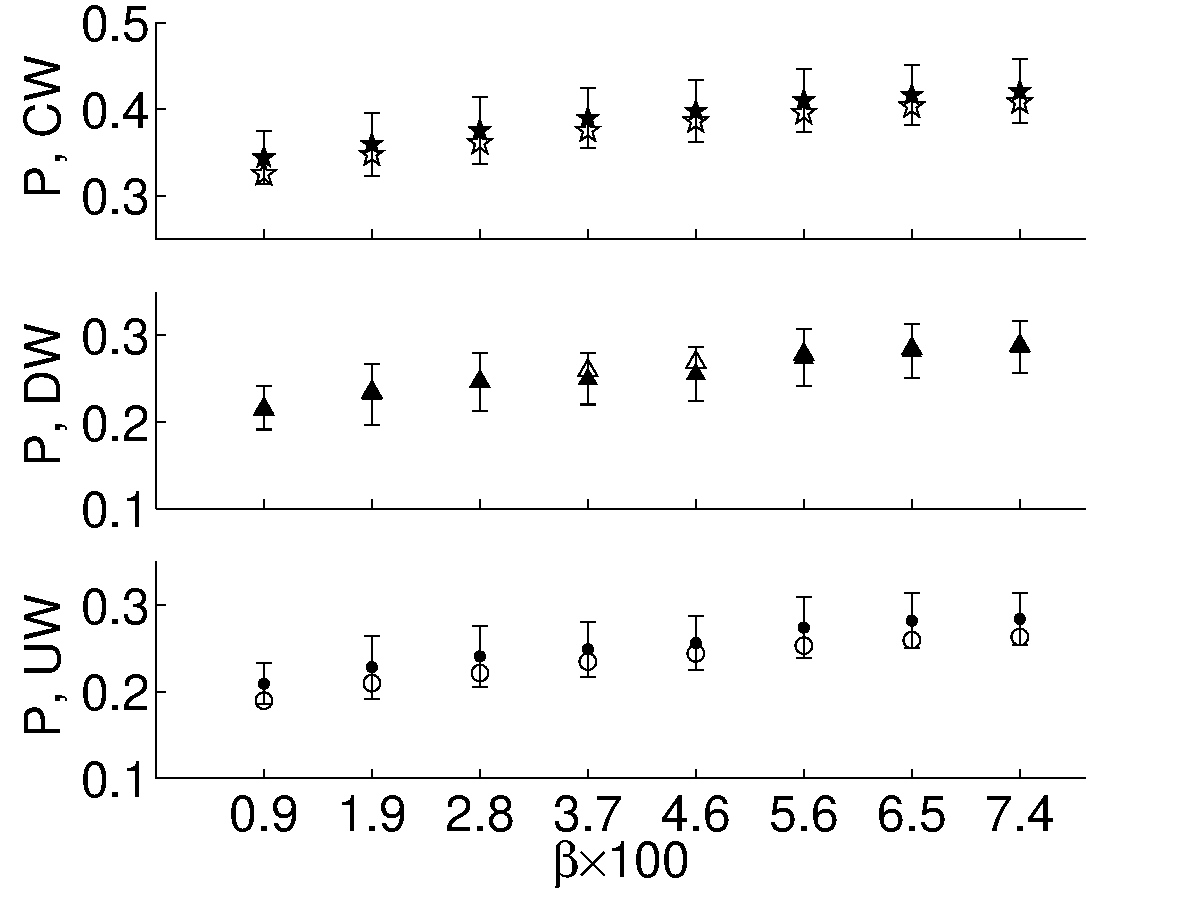
\includegraphics[width=3.25in]{revisedfigures/SupplMatFig1B}
\caption{
{\bf Relationship between success in locating a host and the odor plume shape. } A. Schematic showing the plume measurements that were estimated in order to match the results in B. $w$ is an estimate of maximum plume width, $r_c$ is the host critical radius, $l$ the plume length, and $r_f$ is the average crosswind flight length for a mosquito engaging in the crosswind plume finding behavior. $r_c$ and $r_f$ are constant over all runs, but $w$ and $l$ were averaged over time and over different host arrangements. B. Simulation results for a fixed number of hosts arranged with decreasing density given by the solid markers with $\pm$ one standard deviation (UW = upwind, DW = downwind, CW = crosswind). Open markers use estimates of plume width to predict contact probability. $\beta$ is the area of the host patch divided by the area of the simulation region (the proportion of the domain covered by hosts). As $\beta$ increases, the hosts spread out (i.e., decrease in density) and the number of mosquitoes locating a host increases. The $x$-axis is $\beta$ multiplied by 100 for ease of viewing, since $\beta$ is quite small.}
	\label{fig:denschematic}
\end{figure}

\end{document}
